\section{Results - Research Question 4}

\subsection{Comparing Existing Work: VM vs REF}

\subsubsection{Initial Observations}

\subsubsection{Ordinal Statistics}

\subsubsection{Speedup Analysis}

Since this is a custom benchmark, there exists no readily available comparison with which one can compare execution times.

\subsection{1GB RAM vs 2GB RAM vs 4GB RAM}

We now discuss testing and performance for memory sizes ranging from 1GB to 4GB.  The experience with 512MB was documented with Workload A.

This section describes the results of running the \gls{ycsb} on virtual node networks as described in the methodology.  The summary of execution times are reported in Tables \ref{table:summary_statistics_for_1_config}, \ref{table:summary_statistics_for_3_config}, and \ref{table:summary_statistics_for_6_config}.  For each table, the summary statistics are listed for each amount of memory.

\subsubsection{Initial Observations}

%--fig4--%

It is best to start with a visual inspection of the data represented in Figure \ref{fig:figures-wli_fig4}.  Generally the greater amount of \gls{ram}, the fewer problems one would have with memory overloads, or needing to compact. However, for each sample, it seems that different amount of memory yields the best performance.

By all appearances, it does seem that the 4GB of RAM outperforms the 1GB of RAM and the 2GB of RAM in this case.  It appears that for the 1-node degenerate case, the means could be about equal.  However, for 2, 3, 4, 5, and 6-node clusters, the 4GB seems to have an advantage in the samples here, both in terms of the overall performance in execution time but the deviation from the median as well.

It is not clear from this graph what accounts for the differences.  One possible explanation is compaction: the 4GB nodes never really need to compact.  The amount of data becomes too much for the 1GB and 2GB nodes to hold in the memtables in memory without doing a compaction, and thus allocates, on average, more resources for the triggered compaction events to flush the memtables and get the data onto disk.  To verify this, one could manually inspect sniffed data and/or log compaction events to measure any correlation among memtable size, partition size, node count in the cluster, and frequency of compaction events.  However, if this were the only factor, one would expect to see a particular pattern as the number of nodes in the cluster increased while the number of operations were constant:  low variance from frequent compaction, high variance from periodic compaction, and finally low variance from seldom or nonexistant compaction.  If this is indeed a significant factor, this might be ameliorated by increasing the number of operations, right now set at 10,000, to 100,000 to better represent the steady state.


\begin{figure}[h]
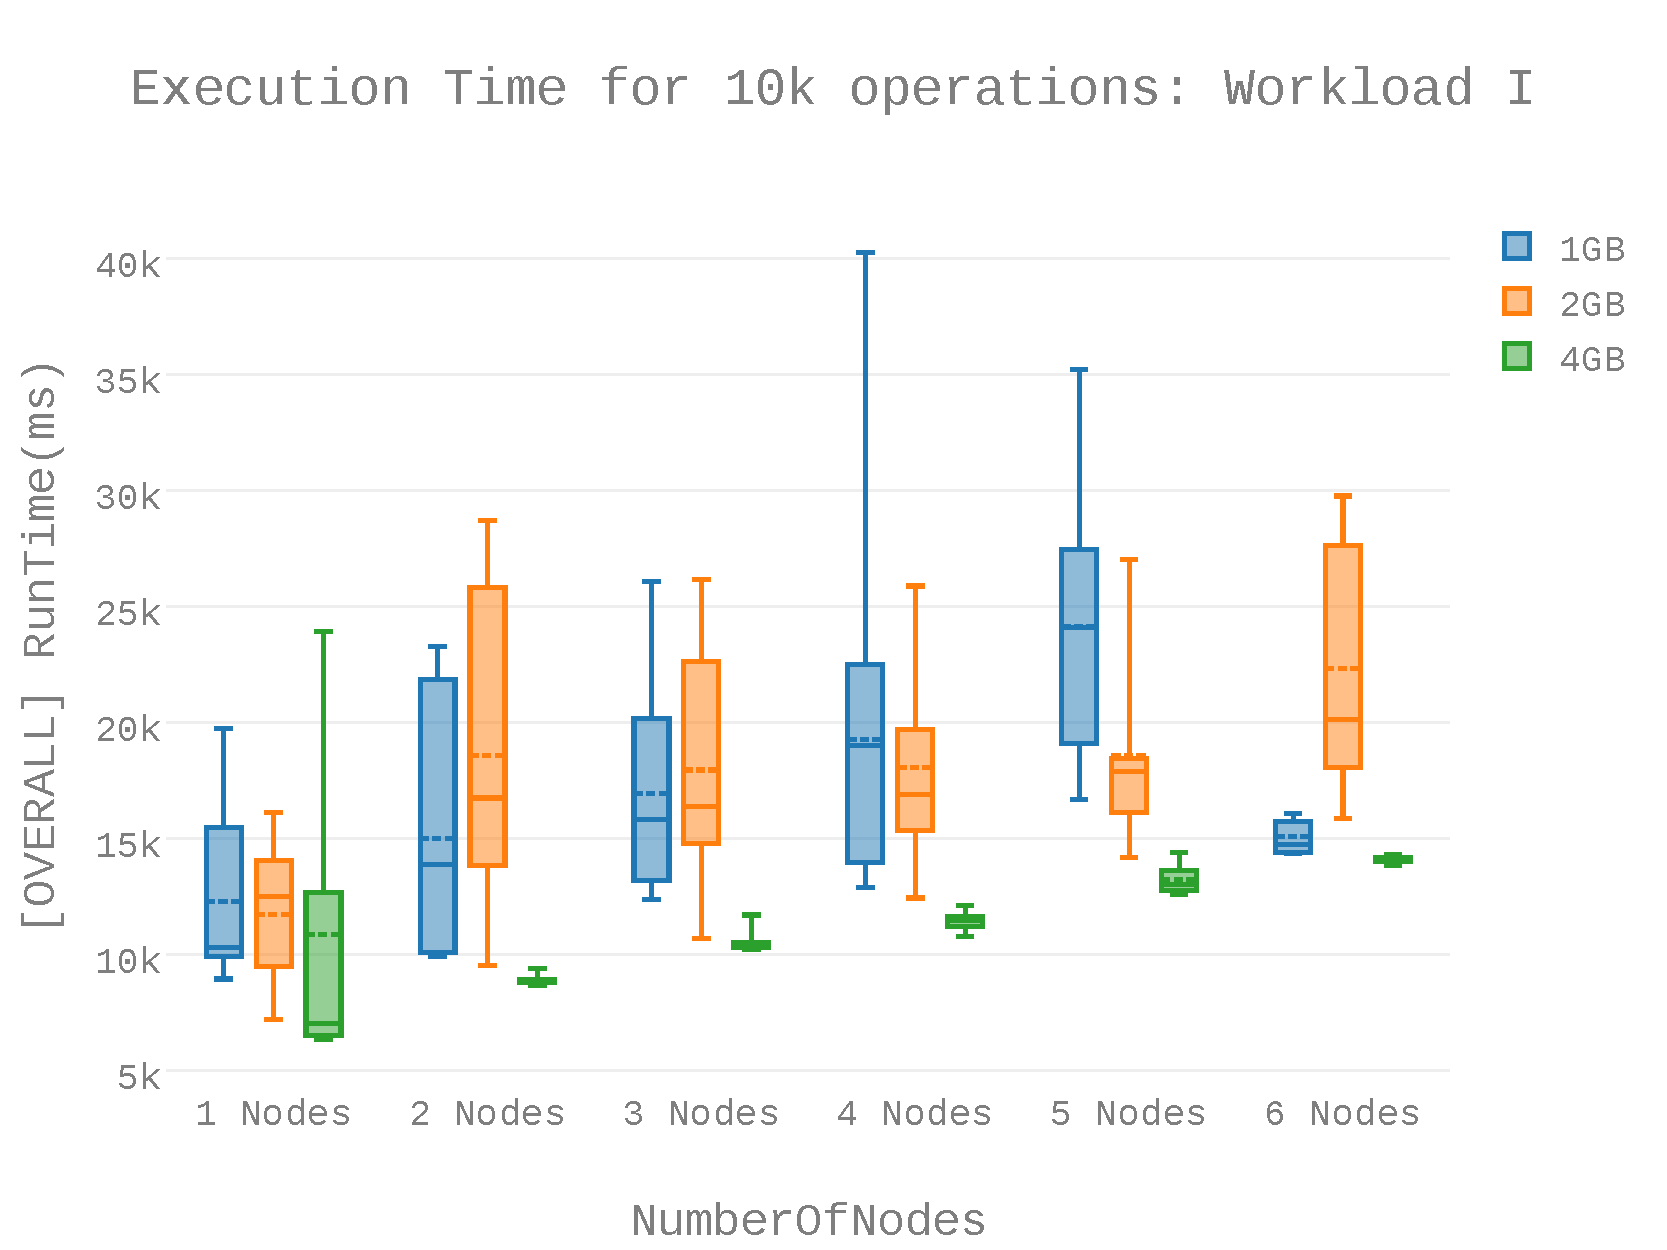
\includegraphics[width=7in]{Figures/figures-wli_fig4.pdf}

\caption{Execution time for virtual machines with 1GB, 2GB, and 4GB of \gls{ram}.  The first 9 trials have been removed in order to filter out the trials representing the cache effect and thus represent the steady state.}

\label{fig:figures-wli_fig4}
\end{figure}

\begin{table}
\begin{tabular}{lrrr}
\toprule
 index &  ram1GB &  ram2GB &  ram4GB \\
\midrule
 count &      21 &      21 &      21 \\
  mean &  356156 & 24989.5 & 25145.5 \\
   std & 6091.15 & 2157.15 &  2121.9 \\
   min &  347166 &   21164 &   19476 \\
   25\% &  350412 &   23254 &   24341 \\
   50\% &  354780 &   25159 &   25195 \\
   75\% &  360472 &   26145 &   26772 \\
   max &  371161 &   29166 &   27919 \\
 range &   23995 &    8002 &    8443 \\
\bottomrule
\end{tabular}
\caption{Summary Statistics for 1-Node Configuration. All values represented fall between 19476.0 ms and 371161.0 ms, or rather within a span of 351685.0 ms.}
\label{table:summary_statistics_for_1_config}
\end{table}
\begin{table}
\begin{tabular}{lrrr}
\toprule
 index &  ram1GB &  ram2GB &  ram4GB \\
\midrule
 count &      21 &      21 &      21 \\
  mean &   23444 & 24544.1 & 23753.2 \\
   std & 1016.02 & 747.466 & 1152.61 \\
   min &   22411 &   23430 &   22828 \\
   25\% &   22813 &   24169 &   23292 \\
   50\% &   23221 &   24399 &   23572 \\
   75\% &   23658 &   24662 &   23892 \\
   max &   26488 &   26396 &   28465 \\
 range &    4077 &    2966 &    5637 \\
\bottomrule
\end{tabular}
\caption{Summary Statistics for 3-Node Configuration. All values represented fall between 22411.0 ms and 28465.0 ms, or rather within a span of 6054.0 ms.}
\label{table:summary_statistics_for_3_config}
\end{table}
\begin{table}
\begin{tabular}{lrrr}
\toprule
 index &  ram1GB &  ram2GB &  ram4GB \\
\midrule
 count &      21 &      21 &      21 \\
  mean & 32493.2 & 31495.7 & 33605.4 \\
   std & 610.462 & 533.638 & 608.798 \\
   min &   31508 &   30551 &   32649 \\
   25\% &   32108 &   31081 &   33199 \\
   50\% &   32448 &   31466 &   33665 \\
   75\% &   32899 &   31896 &   34105 \\
   max &   34101 &   32522 &   34524 \\
 range &    2593 &    1971 &    1875 \\
\bottomrule
\end{tabular}
\caption{Summary Statistics for 6-Node Configuration. All values represented fall between 30551.0 ms and 34524.0 ms, or rather within a span of 3973.0 ms.}
\label{table:summary_statistics_for_6_config}
\end{table}

\subsubsection{Ordinal Statistics}

While Figure \ref{fig:figures-wle_fig4} gives a general sense of what the results look like, the actual summary statistics can be examined in Tables \ref{table:summary_statistics_for_1_config}, \ref{table:summary_statistics_for_3_config}, and \ref{table:summary_statistics_for_6_config}. After filtering out the first nine trials, the results for running 10,000 operations is displayed in Tables \ref{table:summary_statistics_for_1_config}, \ref{table:summary_statistics_for_3_config}, and \ref{table:summary_statistics_for_6_config}.  For each configuration, varying the \gls{ram} of the virtual machine resulted in execution times that fell within 2 seconds of each other.

\subsubsection{Linear Regression for Each Node Cluster Size}

\paragraph{1-Node Cluster}
\paragraph{2-Node Cluster}
\paragraph{3-Node Cluster}
\paragraph{4-Node Cluster}
\paragraph{5-Node Cluster}
\paragraph{6-Node Cluster}

A one-way \gls{anova} was performed with the filtered data, and the \gls{anova} summary tables can be seen in Tables \ref{ram_variance_analysis_workload_a_1_node}, \ref{ram_variance_analysis_workload_a_3_node}, and \ref{ram_variance_analysis_workload_a_6_node} for the 1, 3, and 6 node cases respectively.  For each case, the  p-value is much, much less than 0.05, and thus it can be said that one can be 95\% confident in the decision to fail to reject the null hypothesis, the hypothesis that the means are equal.

\begin{table}
\begin{tabular}{lrrrrr}
\toprule
         Source &          SS &  df &          MS &       F &           p \\
\midrule
 between groups & 1.53468e+12 &   2 & 7.67339e+11 & 49764.9 & 2.50081e-97 \\
  within groups & 9.25156e+08 &  60 & 1.54193e+07 &     nan &         nan \\
          total &  1.5356e+12 &  62 &         nan &     nan &         nan \\
\bottomrule
\end{tabular}
\caption{ANOVA Summary Table for Workload E, 1 Node}
\label{table:ram_variance_analysis_workload_e_1_node}
\end{table}

\begin{table}
\begin{tabular}{lrrrrr}
\toprule
         Source &          SS &  df &          MS &       F &          p \\
\midrule
 between groups & 1.35194e+07 &   2 & 6.75969e+06 & 6.94605 & 0.00193463 \\
  within groups & 5.83902e+07 &  60 &      973170 &     nan &        nan \\
          total & 7.19096e+07 &  62 &         nan &     nan &        nan \\
\bottomrule
\end{tabular}
\caption{ANOVA Summary Table for Workload E, 3 Node}
\label{table:ram_variance_analysis_workload_e_3_node}
\end{table}

\begin{table}
\begin{tabular}{lrrrrr}
\toprule
         Source &          SS &  df &          MS &       F &          p \\
\midrule
 between groups & 4.67783e+07 &   2 & 2.33892e+07 & 68.2518 & 3.4948e-16 \\
  within groups & 2.05614e+07 &  60 &      342689 &     nan &        nan \\
          total & 6.73397e+07 &  62 &         nan &     nan &        nan \\
\bottomrule
\end{tabular}
\caption{ANOVA Summary Table for Workload E, 6 Node}
\label{table:ram_variance_analysis_workload_e_6_node}
\end{table}

Examining the effects of variance in the amount of \gls{ram} allocated the virtual machines does not seem to have a notable impact on performance.  This indicates that, any observed limitation on the Raspberry Pis’ performance is not limited by \gls{ram}, but something else, and that varying \gls{ram} in future tests will not yield significant results.

% Insert something about statistical significance

\subsection{Implementation on Raspberry Pi}

\subsubsection{Initial Observations}

\subsubsection{Ordinal Statistics}

\subsubsection{Scalability of Node Cluster Size}

In a similar fashion, the tests were run on the Raspberry Pi to observe performance.  The spread of each of the tests can be seen in Figure \ref{fig:wle_fig10} and Table \ref{table:wired-results}.  The results, next to one trend for the virtual machines, can be seen in Figure \ref{fig:fig06}. 

\begin{figure}[h]
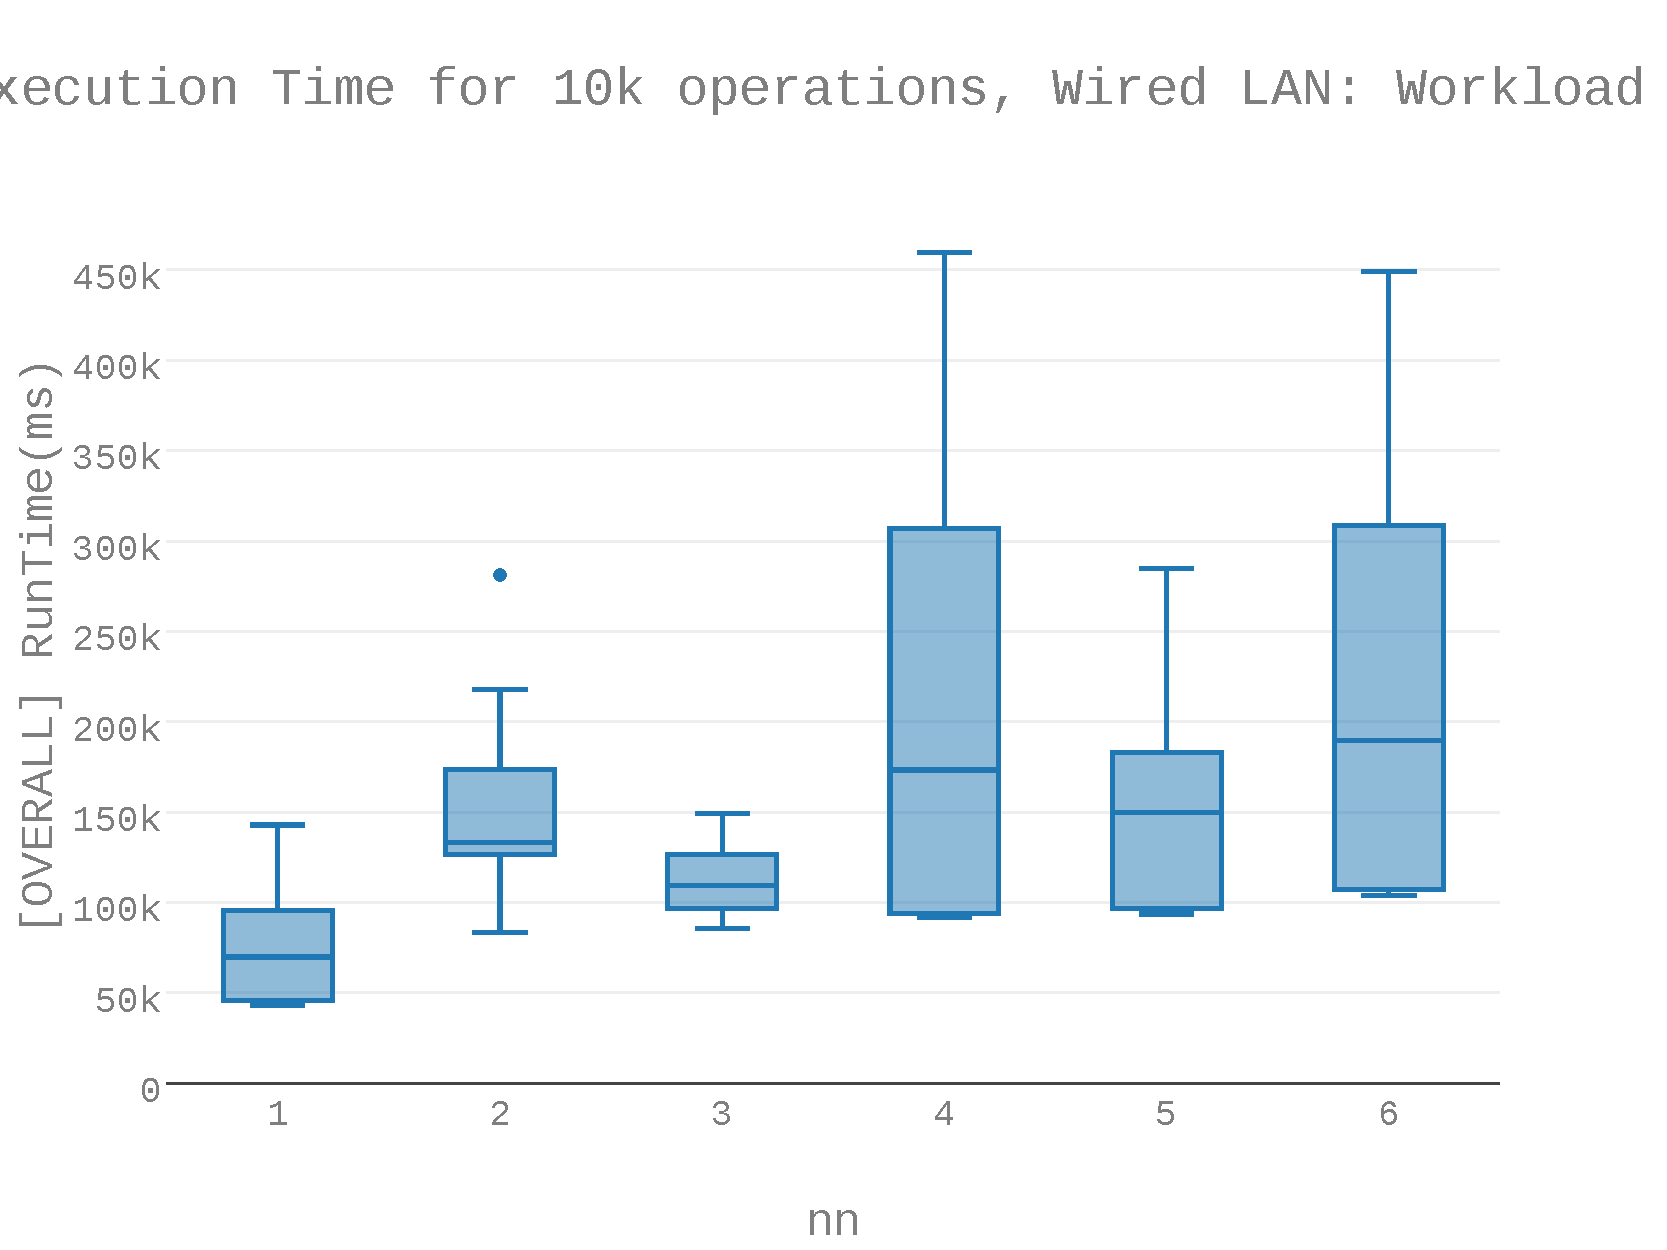
\includegraphics[width=3.5in]{Figures/figures-wle_fig10.pdf}

\caption{Box plot representing the results of the workload applied to wired local area network on the Raspberry Pi platform.}

\label{fig:wle_fig10}
\end{figure}

\begin{figure}[h]
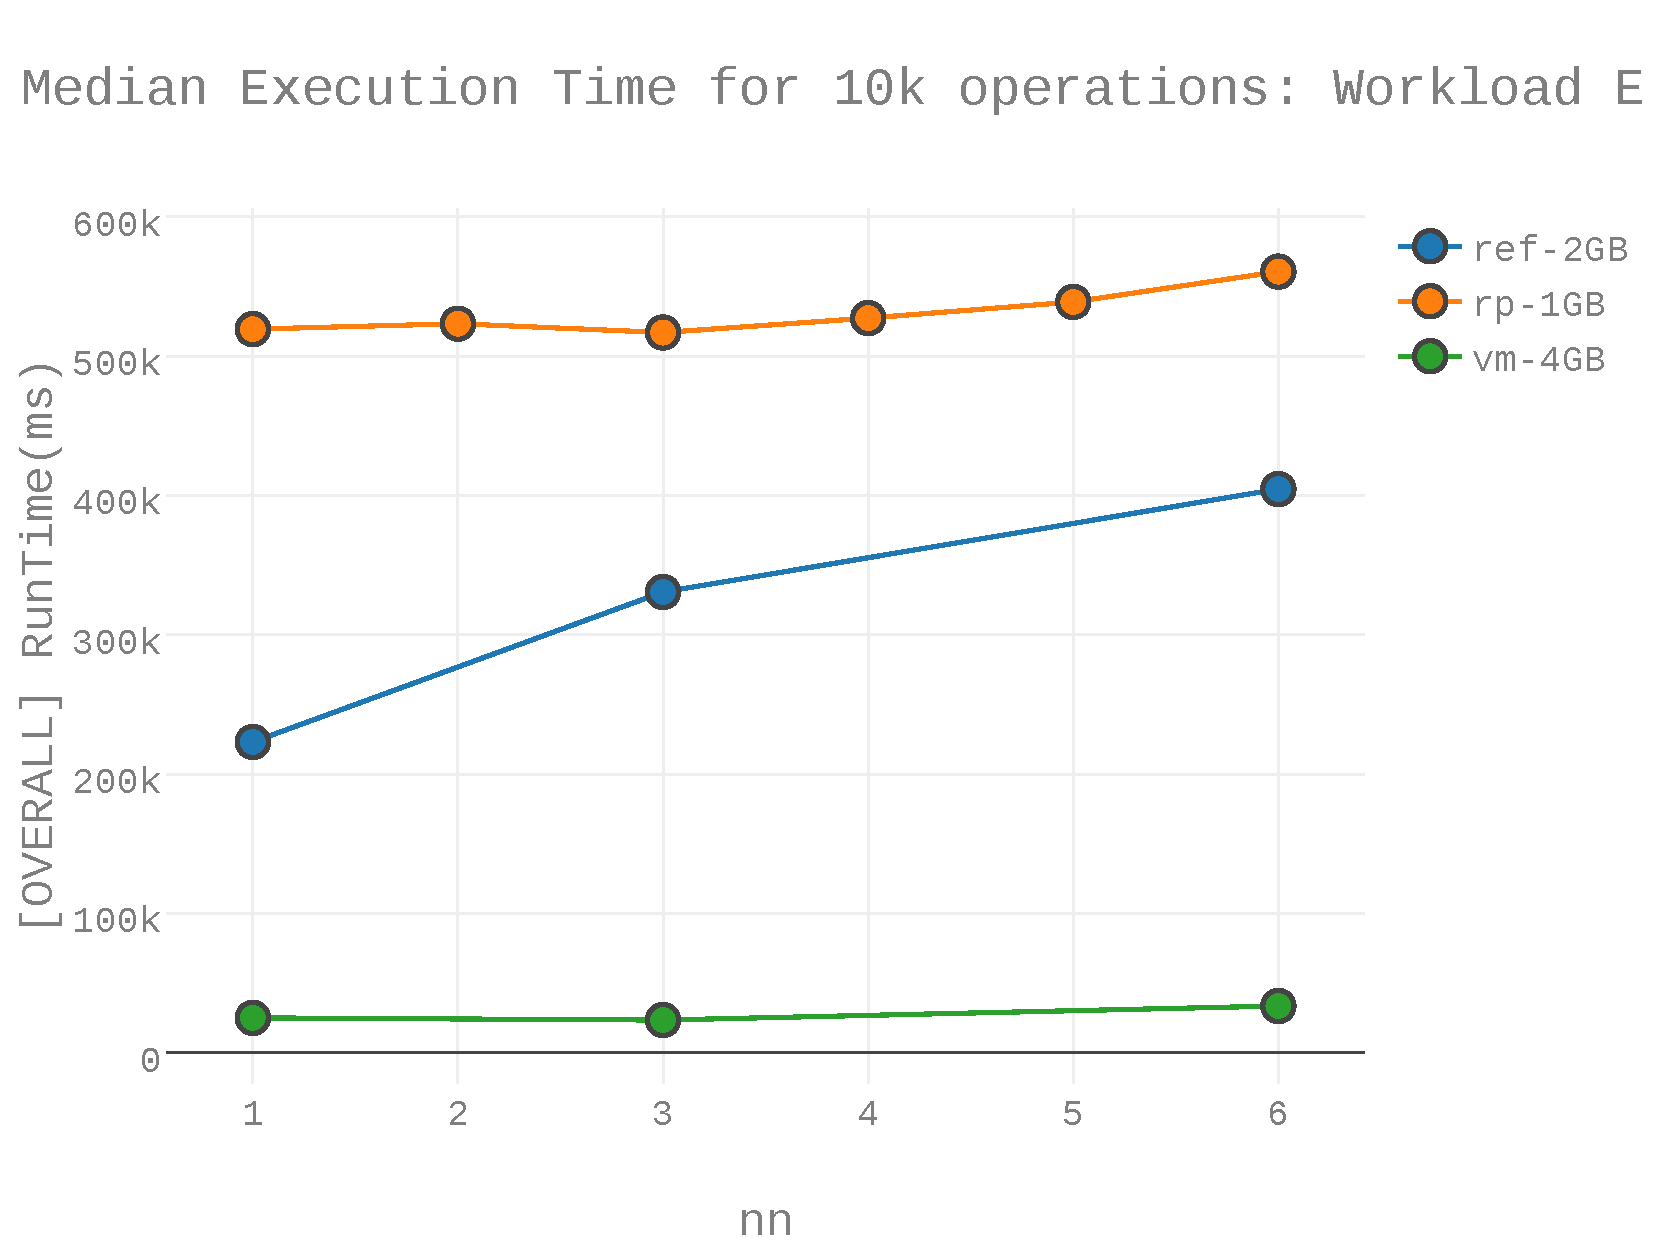
\includegraphics[width=3.5in]{Figures/figures-wle_fig6.pdf}

\caption{Comparison between the Raspberry Pi nodes (rp-1GB), the results reported in \cite{Abramova2014} (ref-2GB), and the virtual nodes with 4GB available \gls{ram} (vm-4GB).}

\label{fig:fig06}
\end{figure}

\begin{table}
\begin{tabular}{lrrr}
\toprule
 index &       1 &       3 &       6 \\
\midrule
 count &      21 &      21 &      21 \\
  mean & 5.2e+05 & 5.2e+05 & 5.6e+05 \\
   std & 2.1e+03 & 5.5e+03 &   3e+03 \\
   min & 5.2e+05 & 5.1e+05 & 5.6e+05 \\
   25\% & 5.2e+05 & 5.1e+05 & 5.6e+05 \\
   50\% & 5.2e+05 & 5.2e+05 & 5.6e+05 \\
   75\% & 5.2e+05 & 5.2e+05 & 5.6e+05 \\
   max & 5.2e+05 & 5.3e+05 & 5.7e+05 \\
 range & 8.3e+03 &   2e+04 &   1e+04 \\
\bottomrule
\end{tabular}
\caption{Summary for Raspberry Pi wired local area network}
\label{table:rp_wired_summary_statistics}
\end{table}

As can be seen from Figure \ref{fig:fig06}, the Raspberry Pi configuration takes considerably more execution time than the virtual machine analogy, which is probably due to the physical nature of the Ethernet connections (propagation delay) and the I/O limitations of the Raspberry Pi hardware.  However, its seemingly similar performance to the reference in \cite{Abramova2014} suggests the \gls{io} for the \gls{sd} Card follows a predictable pattern, and actually seems to outperform the node in \cite{Abramova2014} in the degenerate 1-node case.

For this paragraph, consider the results from \cite{Abramova2014} as the reference.  For a node network of 1, the experimental values fell between 515941.0 ms and 524199.0 ms, inclusive, and all values fell within 301019.0 ms of the reference value of 223180 ms.  For a node network of 3, the experimental values fell between 511997.0 ms and 532260.0 ms, inclusive, and all values fell within 201440.0 ms of the reference value of 330820 ms.  For a node network of 6, the experimental values fell between 555007.0 ms and 565388.0 ms, inclusive, and all values fell within 160728.0 ms of the reference value of 404660 ms.  

\subsection{Raspberry Pi versus the Reference Value}

For {} out of {} nodes, the reference value 

\subsubsection{Initial Observations}

%--fig1--%


\subsubsection{Ordinal Statistics}

\subsubsection{Speedup Analysis}



\subsection{Raspberry Pi versus the Virtual Machine}

\subsubsection{Initial Observations}

\subsubsection{Ordinal Statistics}

\subsubsection{Speedup Analysis}

\subsection{Wireless Links Only}

\subsubsection{Initial Observations}

\subsubsection{Ordinal Statistics}

\subsubsection{Scalability Analysis}

\subsection{Wireless Links versus Wired Links}

\subsubsection{Initial Observations}

\subsubsection{Ordinal Statistics}

\subsubsection{Speedup From Wired Links}

The median value of the corresponding wired experiment will serve as the reference in this paragraph. For a node network of 1, the experimental values fell between 625938.0 ms and 724603.0 ms, inclusive, and all values fell within 204854.0 ms of the reference value of 519749.0 ms.  For a node network of 3, the experimental values fell between 1198600.0 ms and 1458086.0 ms, inclusive, and all values fell within 941493.0 ms of the reference value of 516593.0 ms.  For a node network of 6, the experimental values fell between 260.0 ms and 2018342.0 ms, inclusive, and all values fell within 1459859.0 ms of the reference value of 558483.0 ms.  

\begin{figure}[h]
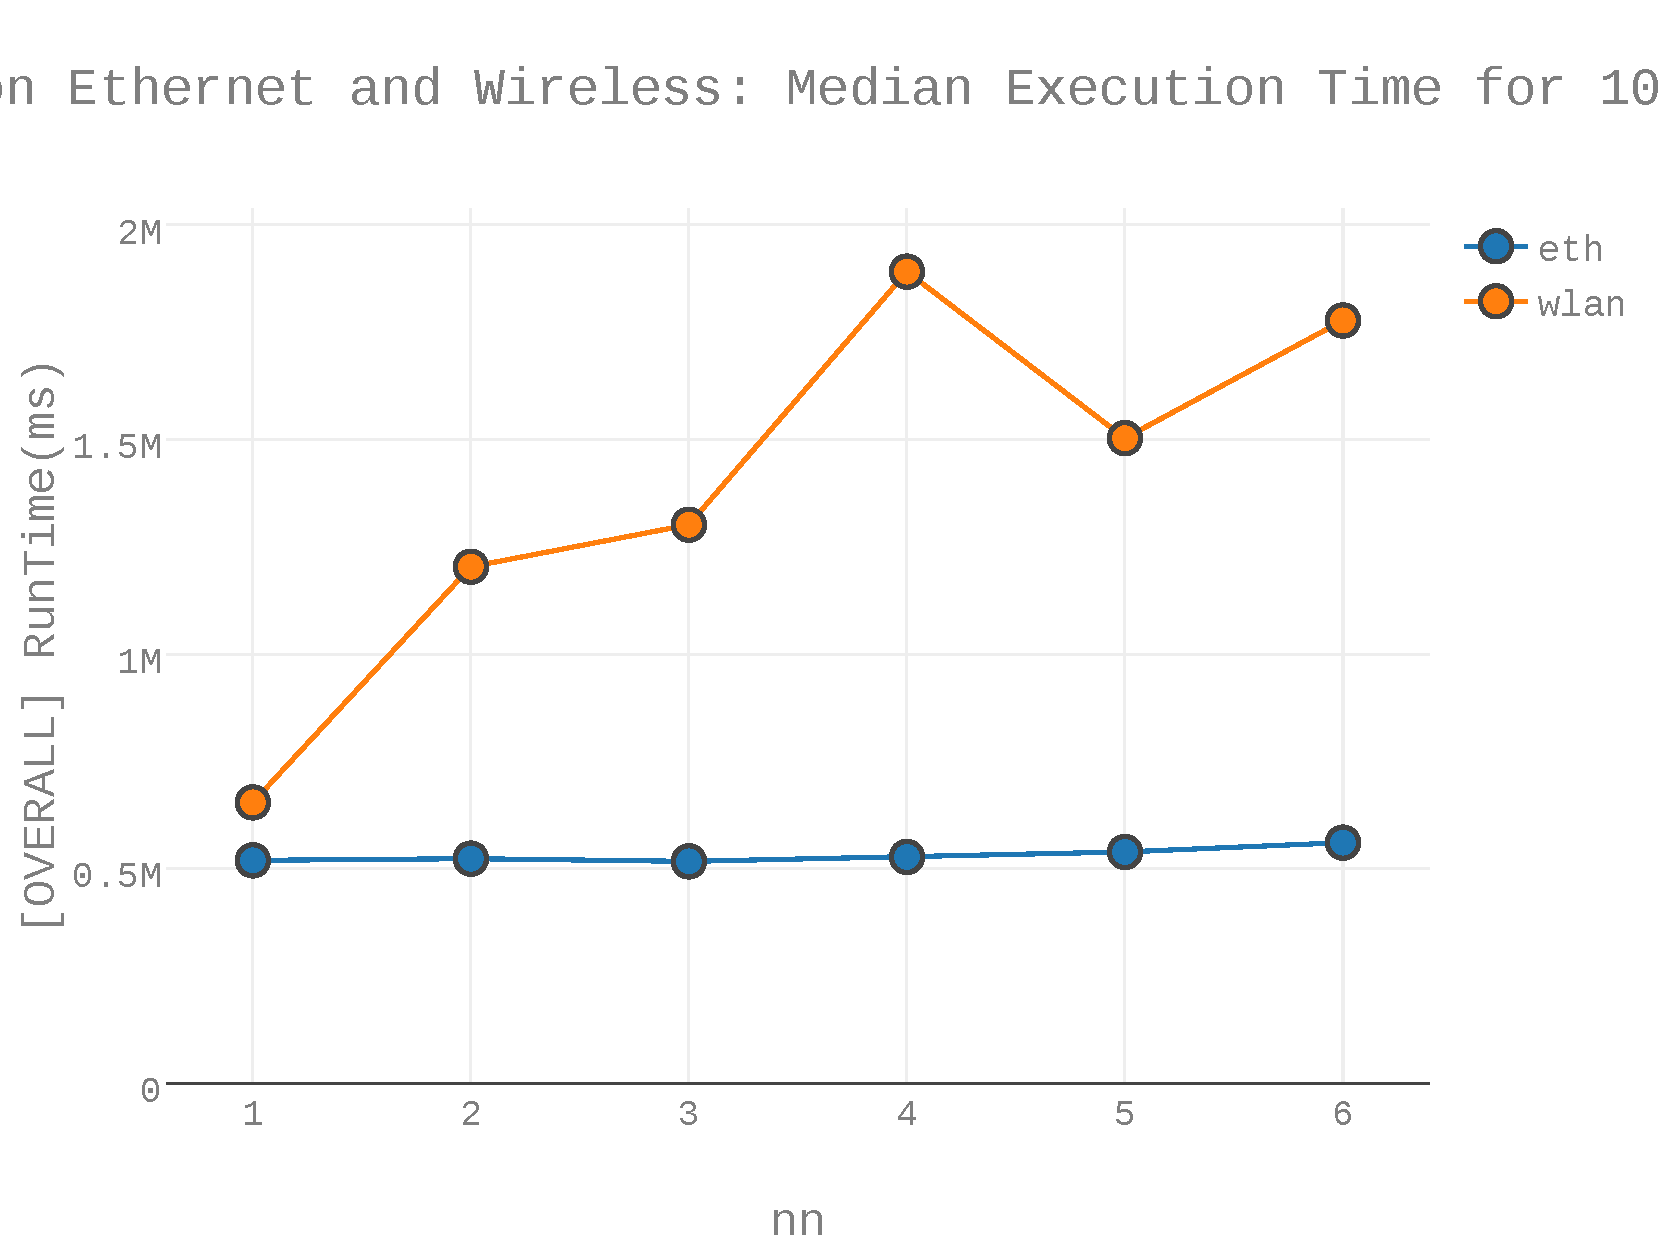
\includegraphics[width=3.5in]{Figures/figures-wle_fig7.pdf}

\caption{Comparison between the Ethernet links (eth) and wireless links (wlan) using the Raspberry Pi nodes.}

\label{fig:fig07}
\end{figure}

Figure \ref{fig:fig07} depicts the two experiments using Raspberry Pis: a wireless LAN (wlan) and an Ethernet LAN (eth).  In Figure \ref{fig:fig07}, as well as previous graphs, one can observe that the the Ethernet LAN effects about 50 seconds of execution time for 10,000 operations.  The initial median execution time for a node on a wireless LAN was found to be double the execution time.

For both configurations, performance takes a hit when transitioning from 1 to 2 nodes, but then increases from 2 nodes to 3 nodes.  From 3 nodes to 4 nodes, the wireless LAN configuration’s performance decreases dramatically, compared to slight increase in the wired Ethernet case.  

\begin{figure}[h]
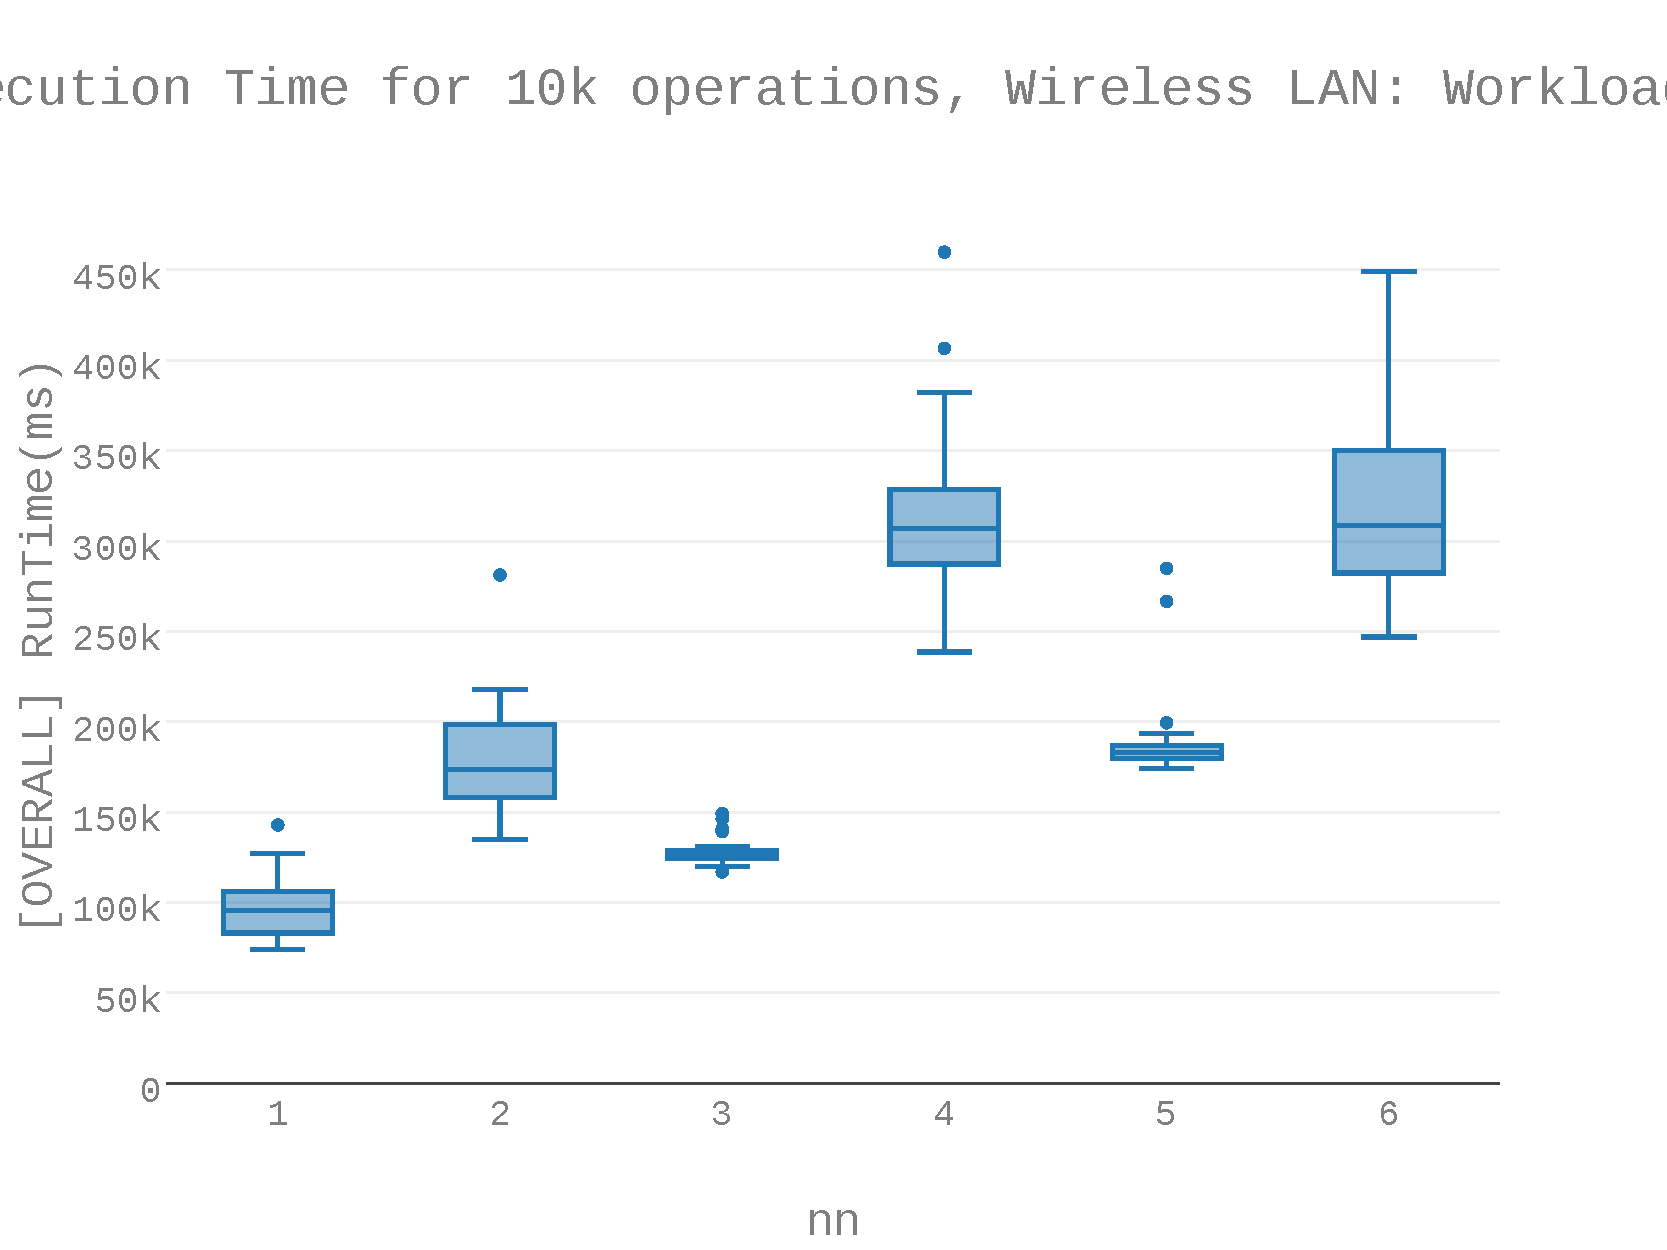
\includegraphics[width=3.5in]{Figures/figures-wle_fig8.pdf}

\caption{Distribution for all 30 trials of execution times where the Raspberry Pi nodes were connected via a wireless \gls{lan}.  Suspected outliers, values more than 3 times the interquartile range, are included as individual points above and below the 'maximum' and 'minimum' bars.}

\label{fig:fig08}
\end{figure}

A summary representation box plot of the results of wireless experimentation is above.  Here, the laptop was connected to the router via an Ethernet cable, and each node was connected to the router on a wireless local area network (LAN).  Suspected outliers, values more than 3 times the interquartile range (IQR) are included as points above and below.
There seems to be an overall increasing trend, while the data seems to oscillate, performing better for odd (1,3,5 node) configurations than for even (2,4,6 node) configurations.  However, there is no current theory behind this anomaly. 

\begin{figure}[h]
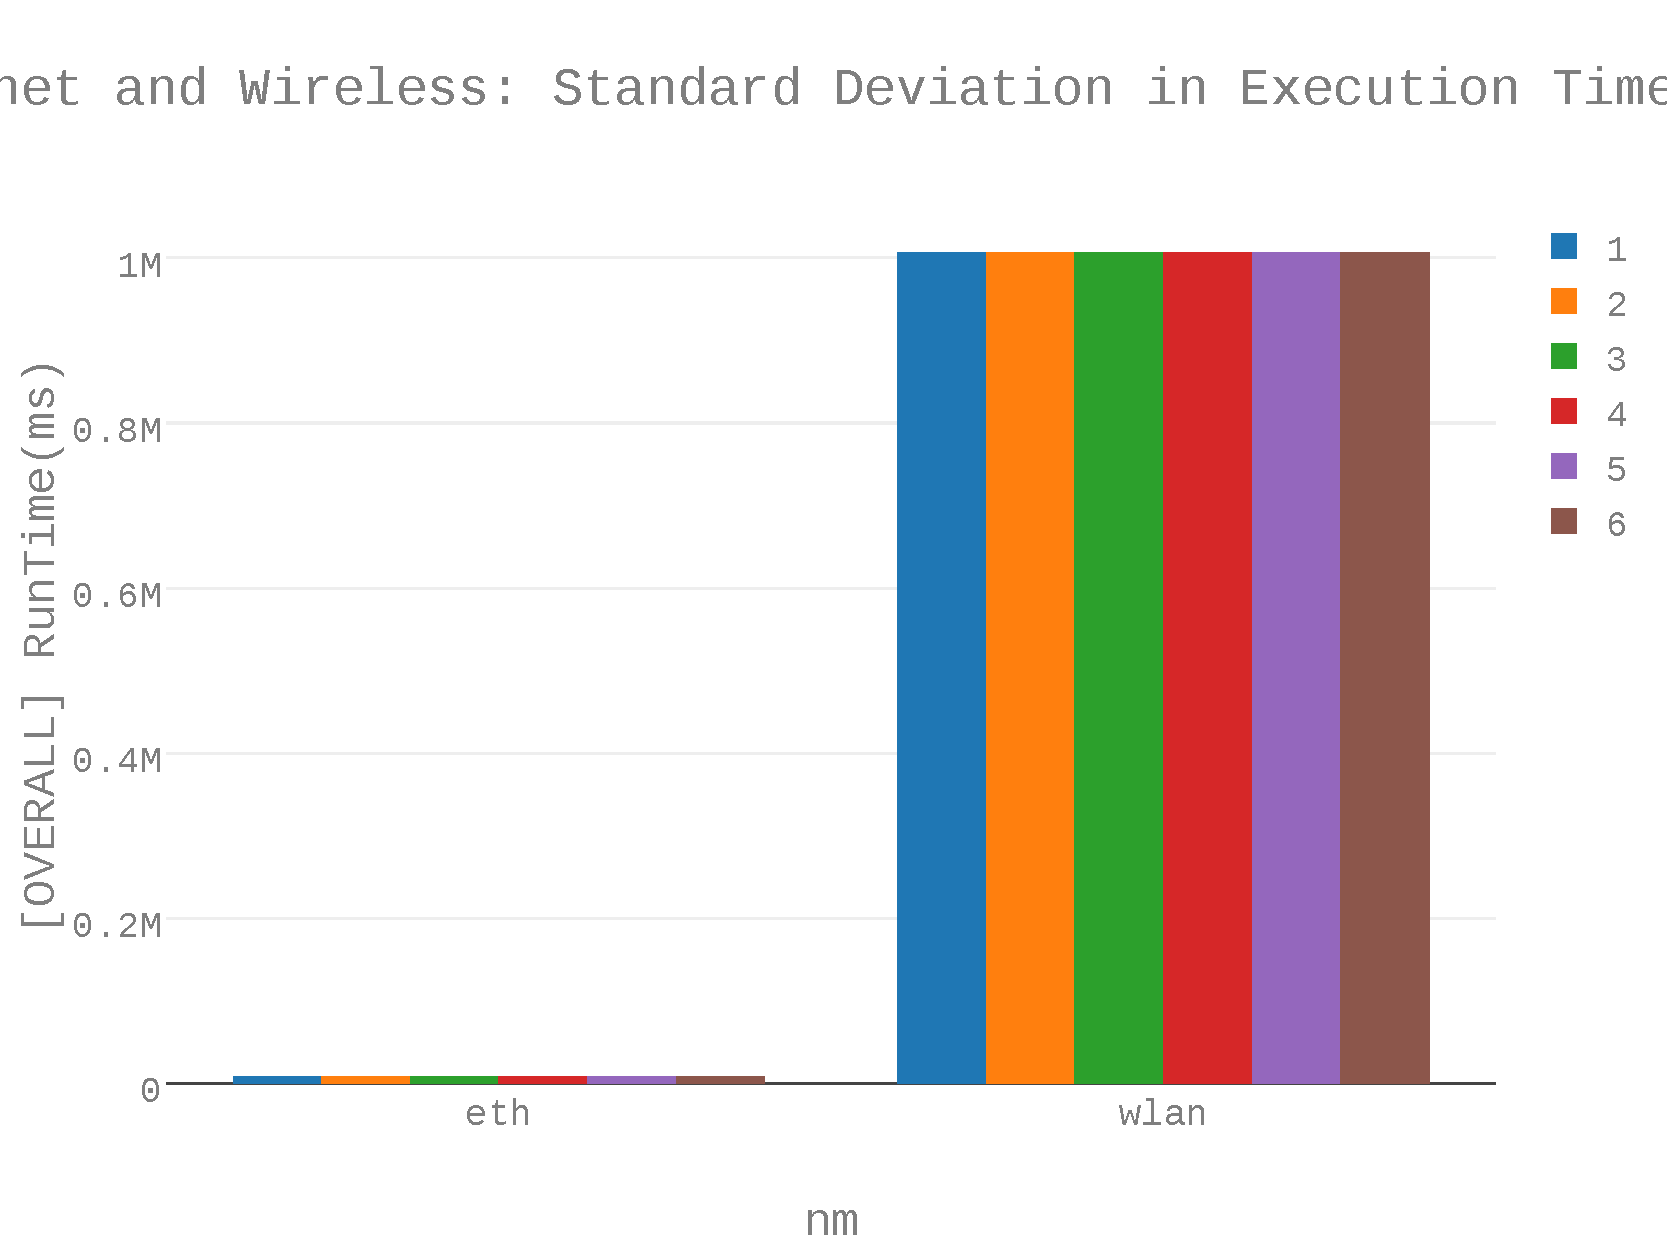
\includegraphics[width=3.5in]{Figures/figures-wle_fig9.pdf}

\caption{This compares the standard deviation in execution times for 10,000 operations of Workload C on the wired (eth) versus the wireless (wlan) configurations for 1 node, 2 nodes, 3 nodes, up through 6 nodes in milliseconds.}

\label{fig:fig09}
\end{figure}

To supplement the box plot, the standard deviation execution times for each set of trials, separated by number of nodes, is depicted in Figure \ref{fig:fig09}.  The difference seen here appears stark, and is overwhelming compared to the variance between 1, 2, 3, 4, 5 and 6 node networks given the same communication method. 

%1)      Reduced performance of Workload A is not statistically significant for the reduced memory sizes of IoT like devices
%2)      When varying platforms, performance for Workload A tracks the performance of the reference paper. For trials performe, reduced performance of Workload A is within 100ms of the reference paper (abramova) for wired implementations.
%3)      When varying communication method, reduced performance of Workload A is within 100ms of the wired platform test (order of magnitude, no greater than 100% increase in delay)
%4)      Reduced performance of Workload C is not statistically significant for the reduced memory sizes of IoT like devices
%5)      When varying platforms, reduced performance of Workload C is within 100ms of the reference paper (abramova) for wired implementations
%6)      When varying communication method, reduced performance of Workload C is within 100ms of the wired platform test
%7)      Reduced performance of Workload E is not statistically significant for the reduced memory sizes of IoT like devices
%8)      When varying platforms, reduced performance of Workload E is within 100ms of the reference paper (abramova) for wired implementations
%9)      When varying communication method, reduced performance of Workload E is within 100ms of the wired platform test
